% !TeX root = ../main.tex

\xchapter{绪论}{Introduction}

\xsection{研究背景与意义}{Background and Motivation}

近年来，以深度学习为代表的人工智能（Artificial Intelligence，AI）技术快速发展，特别是以 Transformer 为核心的大语言模型（Large Language Model，LLM）推动了云端与端侧推理需求的快速增长\cite{vaswani2017attention,zhao2023llm_survey}。在算力需求持续攀升而制程红利逐步放缓的背景下，神经网络处理器（Neural Network Processor Unit，NPU）等领域专用架构（Domain Specific Architecture，DSA）成为提升性能与能效的重要路径\cite{hennessy2019golden}。多核 NPU 在扩展峰值算力的同时，其系统级行为受存储带宽、片上互连与编译调度策略的联合制约，使得架构参数与映射策略的取舍必须在设计早期就联合评估。

\xsubsection{人工智能发展与神经网络芯片算力演进}{AI Progress and NPU Performance Trends}

人工智能的发展呈现出模型规模与任务复杂度持续上升的态势。从早期卷积网络到 Transformer 与大语言模型，参数量与训练算力需求呈指数级增长。为应对这一趋势，产业界持续推出新一代神经网络芯片与其他 DSA 芯片，其峰值算力与能效在代际迭代中不断提升，与上层模型创新形成相互牵引。图\ref{fig:c1_npu_performance_timeline} 给出不同年份的典型神经网络芯片算力增长趋势，数据取自 NVIDIA、Google、华为各代产品的官方规格（16 位浮点 FP16 与 16 位脑浮点 BF16 的峰值算力）。图\ref{fig:c1_dl_training_compute} 给出深度神经网络所需训练计算量随发布年份的指数级增长趋势，直观反映大模型发展对算力需求的持续攀升\cite{sastry2024computing}。模型与硬件以及训练算力两条线索共同说明：AI 工作负载的演进不断抬高对专用算力的需求，而神经网络芯片则通过工艺、架构与多核横向扩展持续提高芯片算力。

\begin{figure}[htbp]
  \centering
  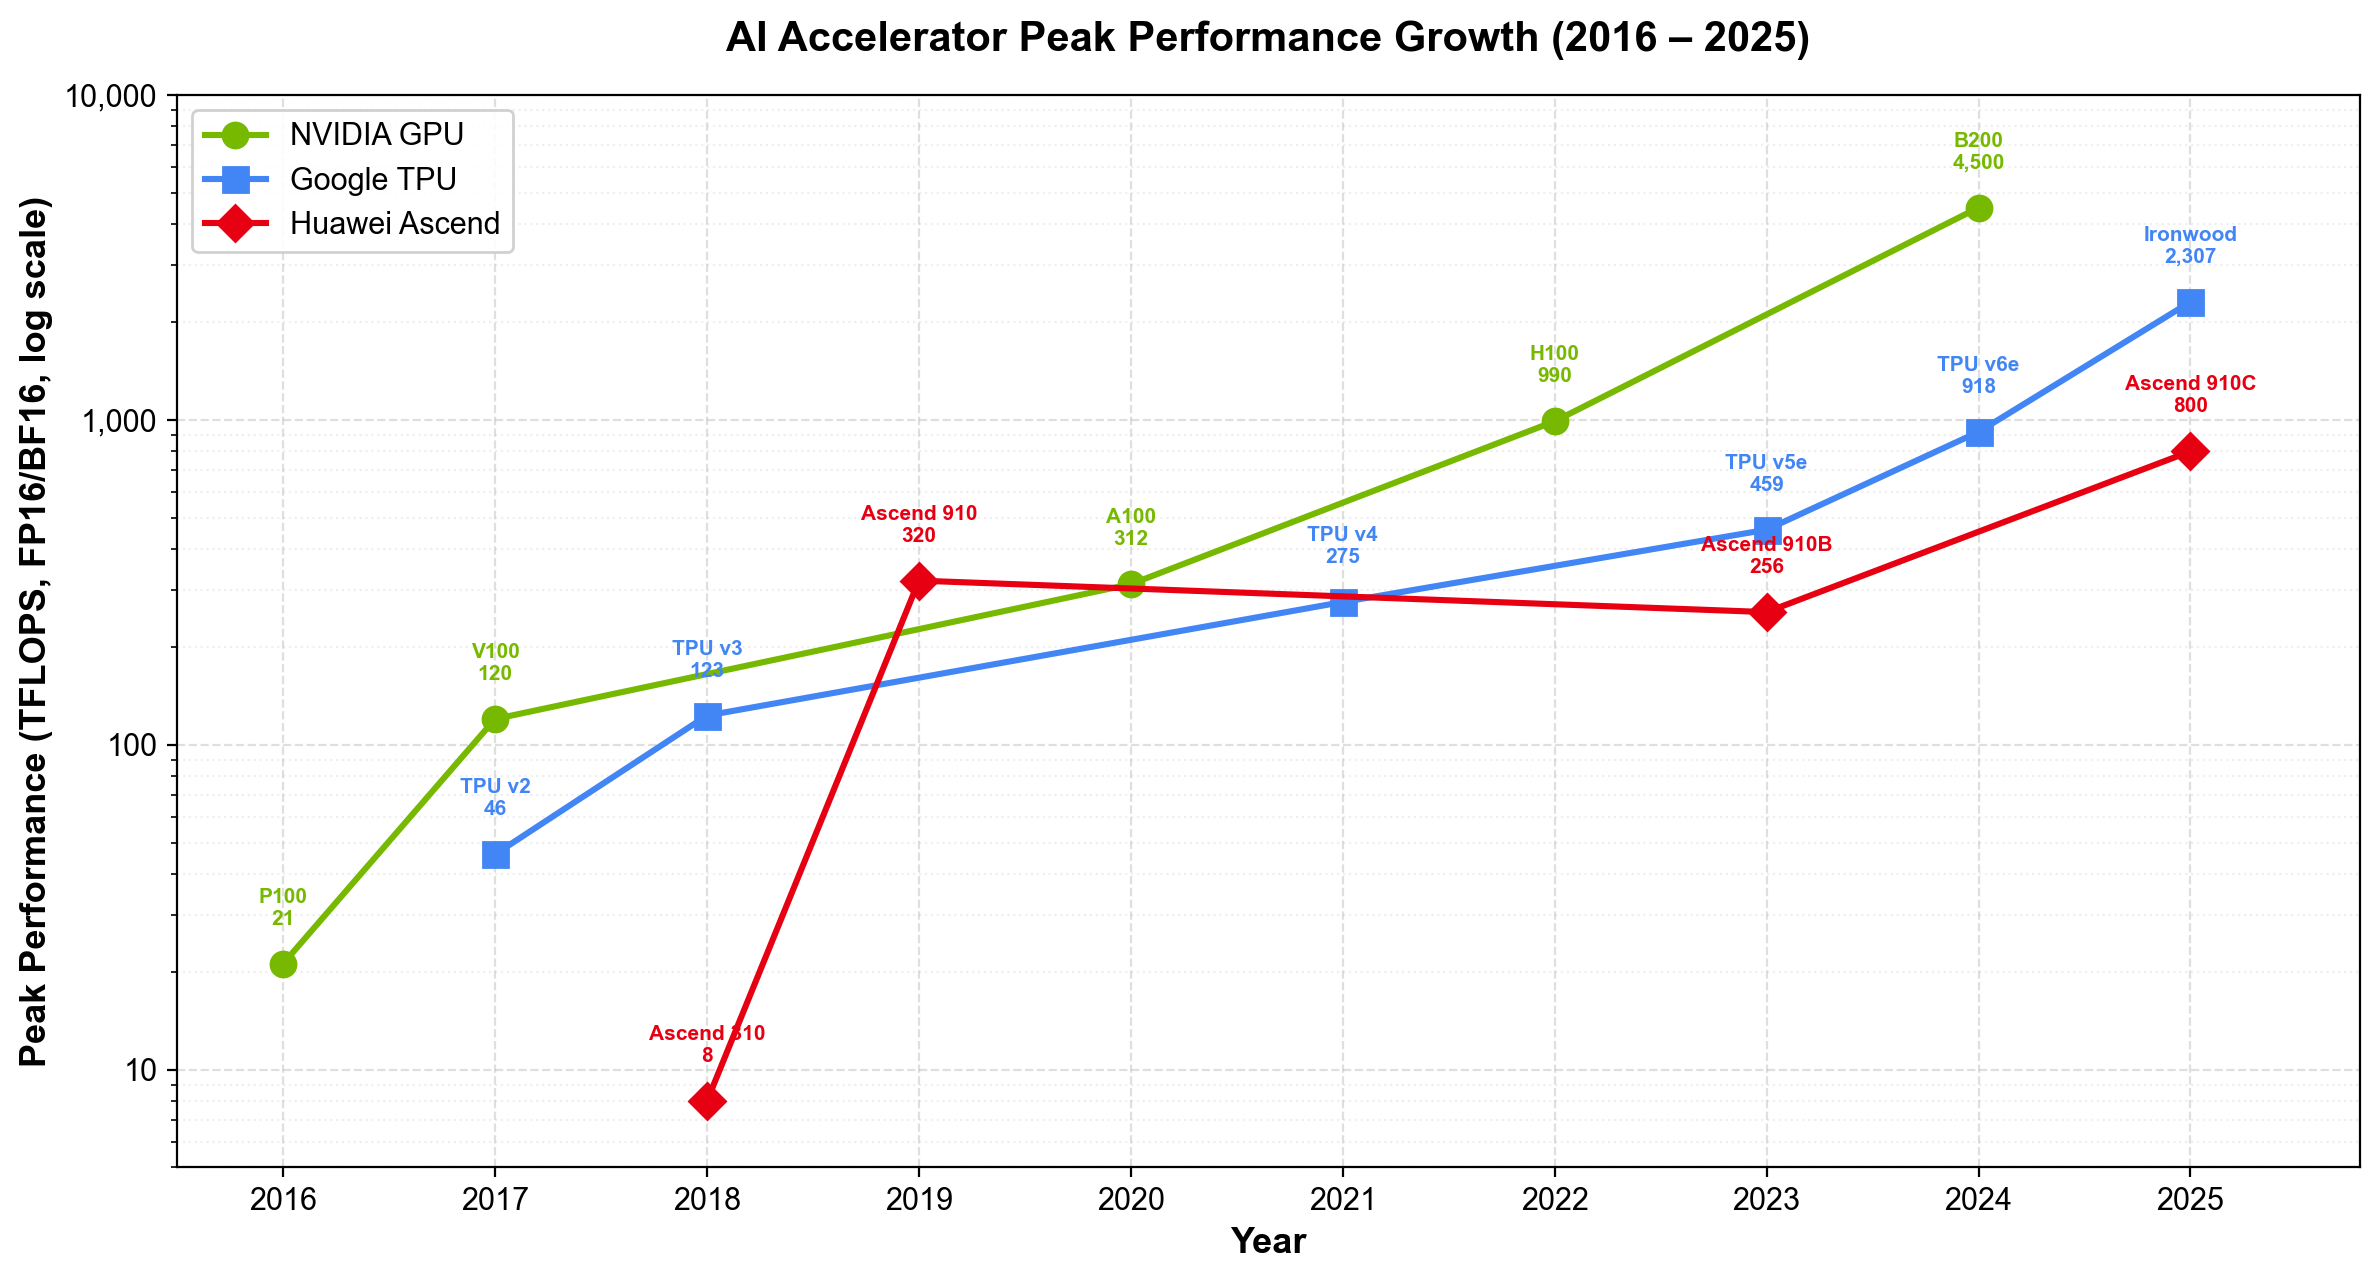
\includegraphics[height=0.3\textheight,keepaspectratio]{Figures/npu_performance_timeline.png}
  \caption{典型神经网络芯片算力规模}
  \label{fig:c1_npu_performance_timeline}
\end{figure}

\begin{figure}[htbp]
  \centering
  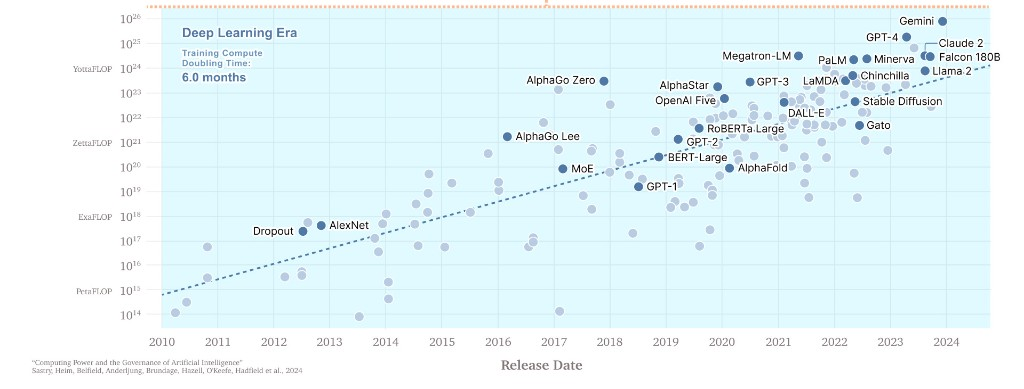
\includegraphics[width=\textwidth]{Figures/dl_training_compute.png}
  \caption{典型神经网络的训练计算量\cite{sastry2024computing}}
  \label{fig:c1_dl_training_compute}
\end{figure}

神经网络芯片是面向神经网络推理与训练而设计的专用硬件加速器，通常具备高并行度的矩阵/向量运算单元、层次化片上存储以及面向数据流的访存与调度机制，与中央处理单元（Central Processing Unit，CPU）或图形处理单元（Graphic Processing Unit，GPU）在编程模型与能效比上形成差异化补充。国内外已有多款代表性神经网络芯片落地。例如 Google 的张量处理单元（Tensor Processing Unit，TPU）系列在云端推理与训练场景中采用脉动阵列作为计算单元的核心架构。华为昇腾、寒武纪思元等国产神经网络芯片在云端与边缘端部署中兼顾多核扩展与软件栈生态。NVIDIA 的推理加速方案（如 NVDLA\cite{veronesi2021nvdla} 等）则与已有 GPU 生态形成协同。Cerebras 则是超大算力多核神经网络芯片的代表产品，如图\ref{fig:c1_cerebras} 所示。Cerebras 是算力需求驱动下从单核到多核、从单芯片到晶圆级扩展的典型形态之一，将整片晶圆集成为单一大规模计算平面，将多核扩展推向物理极限。这些芯片在单核算力、多核互联与存储层次上形态各异，但共同面临算力增长时的系统级瓶颈问题。随着单芯片算力规模受限，多核阵列成为扩展神经网络芯片算力与兼顾能效的主流方向，但也引入了片上网络拥塞、主存带宽瓶颈与跨核调度复杂度高等系统级挑战\cite{gholami2024aimemorywall,cai2024gemini}。

\begin{figure}[htbp]
  \centering
  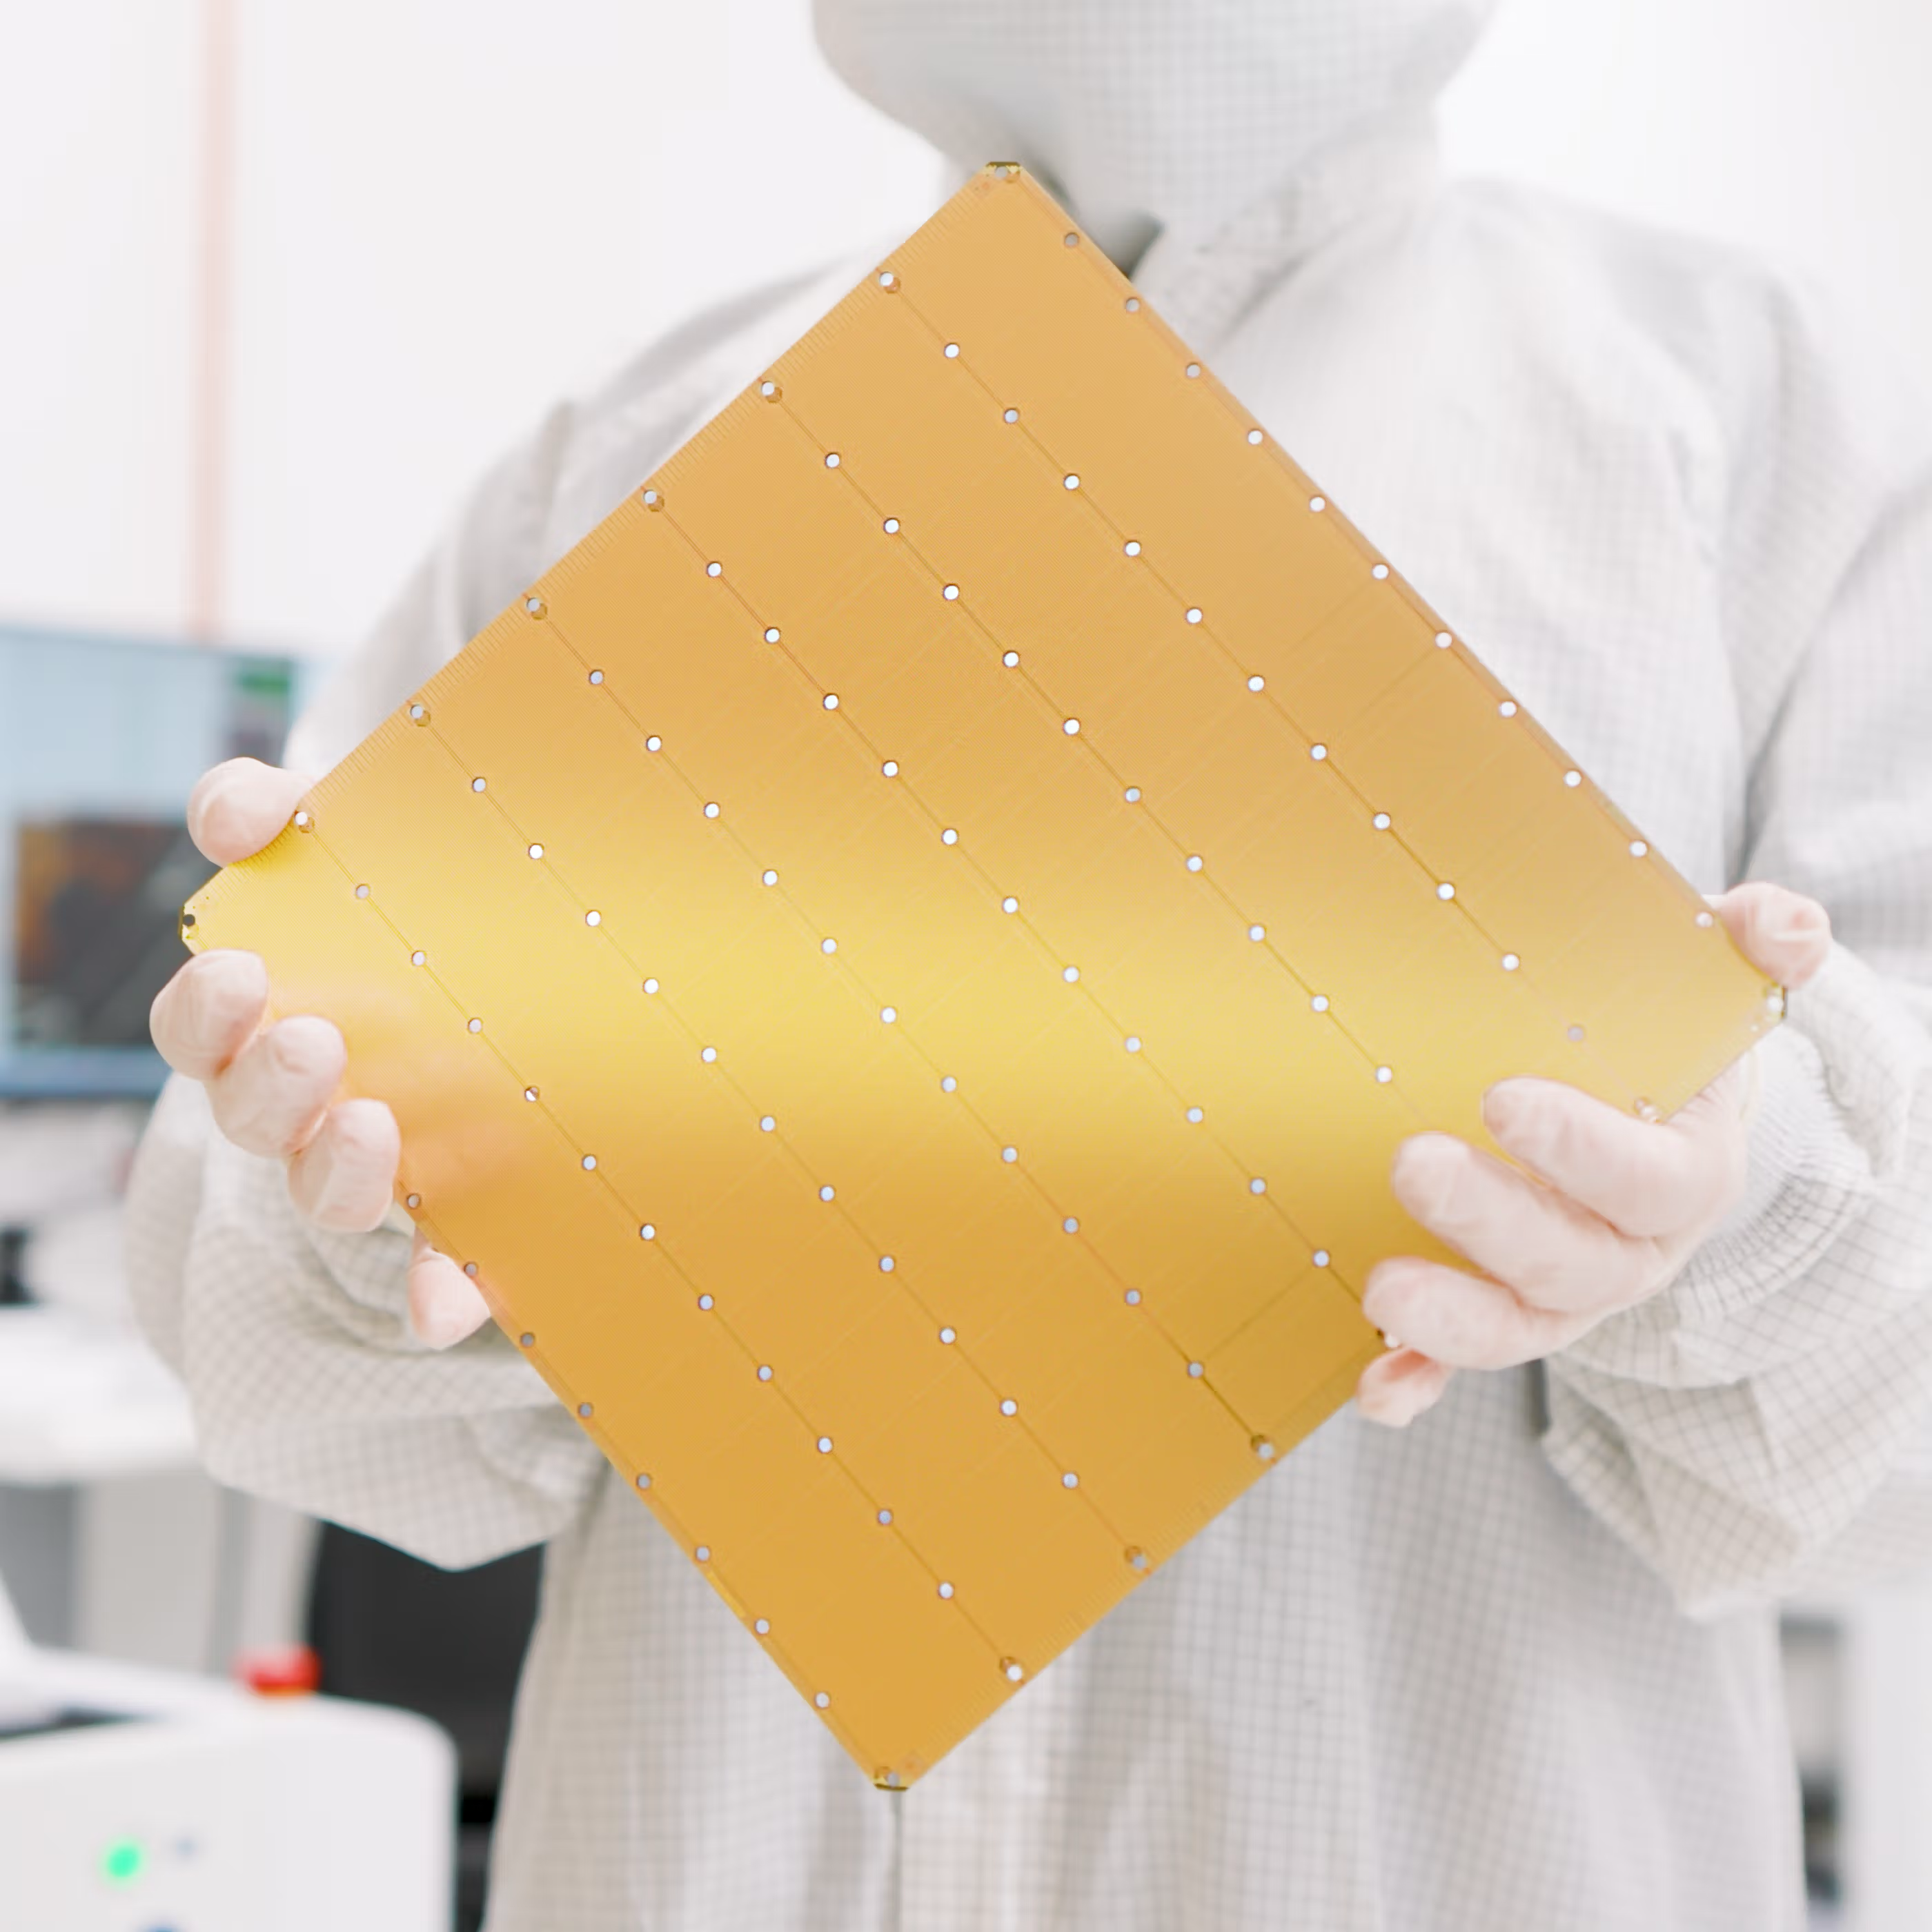
\includegraphics[width=0.35\textwidth]{Figures/cerebras.png}
  \caption{Cerebras 晶圆级引擎示意图\cite{cerebras_wse}}
  \label{fig:c1_cerebras}
\end{figure}

在先进工艺下，芯片的流片成本高昂且迭代周期长。为了在设计早期进行架构探索与软硬件协同优化，构建端到端、高保真且可扩展的多核神经网络芯片模拟平台具有重要意义。一方面，周期级模拟能够在统一时间轴下刻画计算、通信与存储的竞争行为，从而定位端到端性能瓶颈。另一方面，模拟平台为映射策略、互连配置与存储参数的设计空间探索（Design Space Exploration，DSE）提供低成本试错环境\cite{jin2024onnxim,luo2023ramulator2}。从单核到多核阵列、单芯片再到晶圆级形态，算力扩展不断伴随着系统级瓶颈。

\xsubsection{多核神经网络芯片架构设计挑战}{Challenges in Multi-core Neural Network Chip Design}

随着单核神经网络芯片算力逼近工艺与功耗极限，业界普遍采用多核阵列的方式横向扩展峰值吞吐。然而，多核架构在带来线性算力增长的同时，也引发了一系列系统级瓶颈。在扩展的极端形态上，晶圆级引擎等设计将通信、存储与调度挑战更为集中地显现。总体而言，多核神经网络芯片的端到端性能受制于存储、通信与编译调度三个维度的“墙效应”，三者相互耦合，共同决定了实际可达的有效利用率。

第一类瓶颈是“存储墙”，即计算单元的峰值吞吐增速远超片外存储（Dynamic Random-Access Memory，DRAM）的带宽增速所导致的性能瓶颈。在多核神经网络芯片系统中，这一问题尤为突出：当核心数量线性扩展时，峰值算力线性增长，但共享的 DRAM 带宽难以同步扩展，使得存储带宽成为系统吞吐的瓶颈\cite{gholami2024aimemorywall}。大语言模型进一步放大了上述矛盾。推理侧的自回归解码在逐词元（Token）生成时难以像预填（Prefill）阶段那样充分摊薄通用矩阵乘（General Matrix Multiply，GEMM）类算子，需反复从高带宽存储器（High Bandwidth Memory，HBM）或其他类型 DRAM 拉取海量权重，并伴随键值缓存（Key-Value Cache，KV Cache）的读写与扩容。训练侧除前向与反向中的激活与梯度外，还需保存优化器状态与检查点。从屋顶线（Roofline）模型\cite{williams2009roofline} 视角看，如图\ref{fig:c1_roofline}，硬件峰值算力与存储带宽在算术强度（每字节访存所完成的浮点运算次数，FLOPs/Byte，其中 FLOPs 即 Floating-point Operations）维度上共同构成性能上界：工作点的算术强度低于脊点 $\mathrm{AI}_\mathrm{ridge}$ 时性能受存储带宽约束（斜线段），高于脊点时受峰值算力约束（水平段）。大模型推理中的部分注意力、归一化与逐元素算子，以及解码阶段整体较低的批次并行度，常使实际工作点更接近访存受限区。文献\parencite{dao2022flashattention,dao2023flashattention2}提出的快速注意力（FlashAttention）系列算法通过分块计算降低片外访存，文献\parencite{kwon2023pagedattention}提出的分页式注意力（PagedAttention）算法通过分页式 KV Cache 管理缓解碎片。然而在多核与多租户场景下，DRAM 通道争用与行缓冲冲突仍使实际可用带宽显著低于标称峰值。这种竞态行为只有通过周期级的存储控制器模拟才能准确刻画。

\begin{figure}[htbp]
  \centering
  \resizebox{0.82\textwidth}{!}{%
  \begin{tikzpicture}[>=stealth, line cap=round, line join=round, font=\small]
    \coordinate (O) at (0,0);
    \coordinate (ridge) at (4.2,5.5);
    \coordinate (end) at (9.2,5.5);
    \draw[->, thick] (O) -- (10.2,0) node[below] {算术强度（FLOPs/Byte）};
    \draw[->, thick] (O) -- (0,6.8) node[left, align=center] {性能\\（FLOPs/s）};
    \draw[very thick, blue!65!black] (O) -- (ridge) -- (end);
    \draw[dashed, gray!65] (ridge |- O) -- (ridge);
    \node[below, font=\footnotesize] at (ridge |- O) {$\mathrm{AI}_\mathrm{ridge}$};
    \node[text=blue!65!black, align=center] at (2.05,4.55) {访存受限区};
    \node[text=blue!65!black] at (7.6,4.85) {算力受限区};
    % 典型 LLM 推理阶段示意工作点（相对位置，非实测）：Decode 算术强度较低、贴近带宽斜线。Prefill 批处理提示、GEMM 更易摊薄，工作点更靠右并常接近算力平顶
    \coordinate (pt_decode) at (1.45,{5.5/4.2*1.45});
    \coordinate (pt_prefill) at (6.75,5.5);
    \fill[orange!80!black] (pt_decode) circle (2.8pt);
    \fill[teal!70!black] (pt_prefill) circle (2.8pt);
    \node[font=\footnotesize, anchor=south west, inner sep=1pt, text=orange!85!black] at ($(pt_decode)+(0.12,0.22)$) {Decode};
    \node[font=\footnotesize, anchor=south, inner sep=1pt, text=teal!60!black] at ($(pt_prefill)+(0,0.28)$) {Prefill};
  \end{tikzpicture}%
  }
  \caption{屋顶线模型示意图\cite{williams2009roofline}}
  \label{fig:c1_roofline}
\end{figure}

第二类瓶颈是“通信墙”，多核神经网络芯片通过片上网络（Network-on-Chip，NoC）实现核间数据传输。当并行策略将神经网络层的计算分配到多个核心上时，层间的中间激活值、部分和以及权重分片等数据需要经由 NoC 在核心之间搬运，随着核心数量增加和互连直径增大，通信开销呈现超线性增长趋势\cite{jiang2013booksim,flooonoc2024}。在张量并行模式下，全局规约（AllReduce）或全局收集（AllGather）等集合通信操作需在每一层结束时同步全部核心的结果，链路拥塞与仲裁等待会显著放大尾延迟。在流水并行模式下，流水气泡的大小与核间传输延迟直接相关。NoC 的拓扑结构、路由算法、虚拟通道数量、微片（Flit）大小与注入队列深度等参数共同影响吞吐与延迟特性，不同参数配置下的性能差异可达数倍，且与具体流量模式紧密相关，难以通过解析模型精确预测。

第三类瓶颈是“编译与调度墙”，多核神经网络芯片的编译与调度面临的核心困难在于：工作负载到硬件的映射空间随核心数量和网络层数呈指数增长，且映射质量与底层硬件参数强耦合\cite{cai2024gemini}。编译器需要决定每一层（或算子组）的空间切分策略、时序调度顺序与数据布局，每一项选择都会影响计算效率、通信开销与存储占用。文献\parencite{cai2024gemini}提出的 Gemini 调度器给出了层流水空间映射编码与模拟退火搜索框架，文献\parencite{lattner2021mlir,qualcomm2026hexagonmlir}提出的 MLIR 等多层中间表示基础设施也为神经网络芯片后端提供了统一抽象。然而编译器生成的调度方案的实际效果往往取决于运行时 NoC 拥塞、DRAM 排队延迟等系统行为，单纯依靠编译期的代价模型难以准确评估。这就产生了编译与执行之间的语义鸿沟：代价模型通常基于峰值带宽、理想延迟等静态假设，而实际系统中的资源竞争与时序交互是动态且非线性的。

综合来看，上述三类挑战并非彼此独立，而是高度耦合的。增加 DRAM 通道数虽然缓解存储墙，但可能因 NoC 上的存储请求流量增加而加剧通信墙。调整映射策略以减少跨核通信，可能导致单核 SRAM（Static Random Access Memory，静态随机存取存储器）不足而增加 DRAM 溢写，反过来加重存储墙。这种多维耦合特性使得对任何单一子系统的孤立优化都可能在系统层面产生意外的负面效果。图\ref{fig:c1_three_walls}概括了上述三类瓶颈及其耦合关系。因此，构建一个能够将计算、通信与存储三者纳入统一时间轴的端到端周期级模拟平台，成为多核神经网络芯片架构设计的关键需求。这样的模拟器不仅能够定位性能瓶颈的根因，更能为编译器与架构师提供定量可靠的反馈，支撑大规模设计空间探索。上述需求构成了本文研究工作的出发点。

\begin{figure}[htbp]
  \centering
  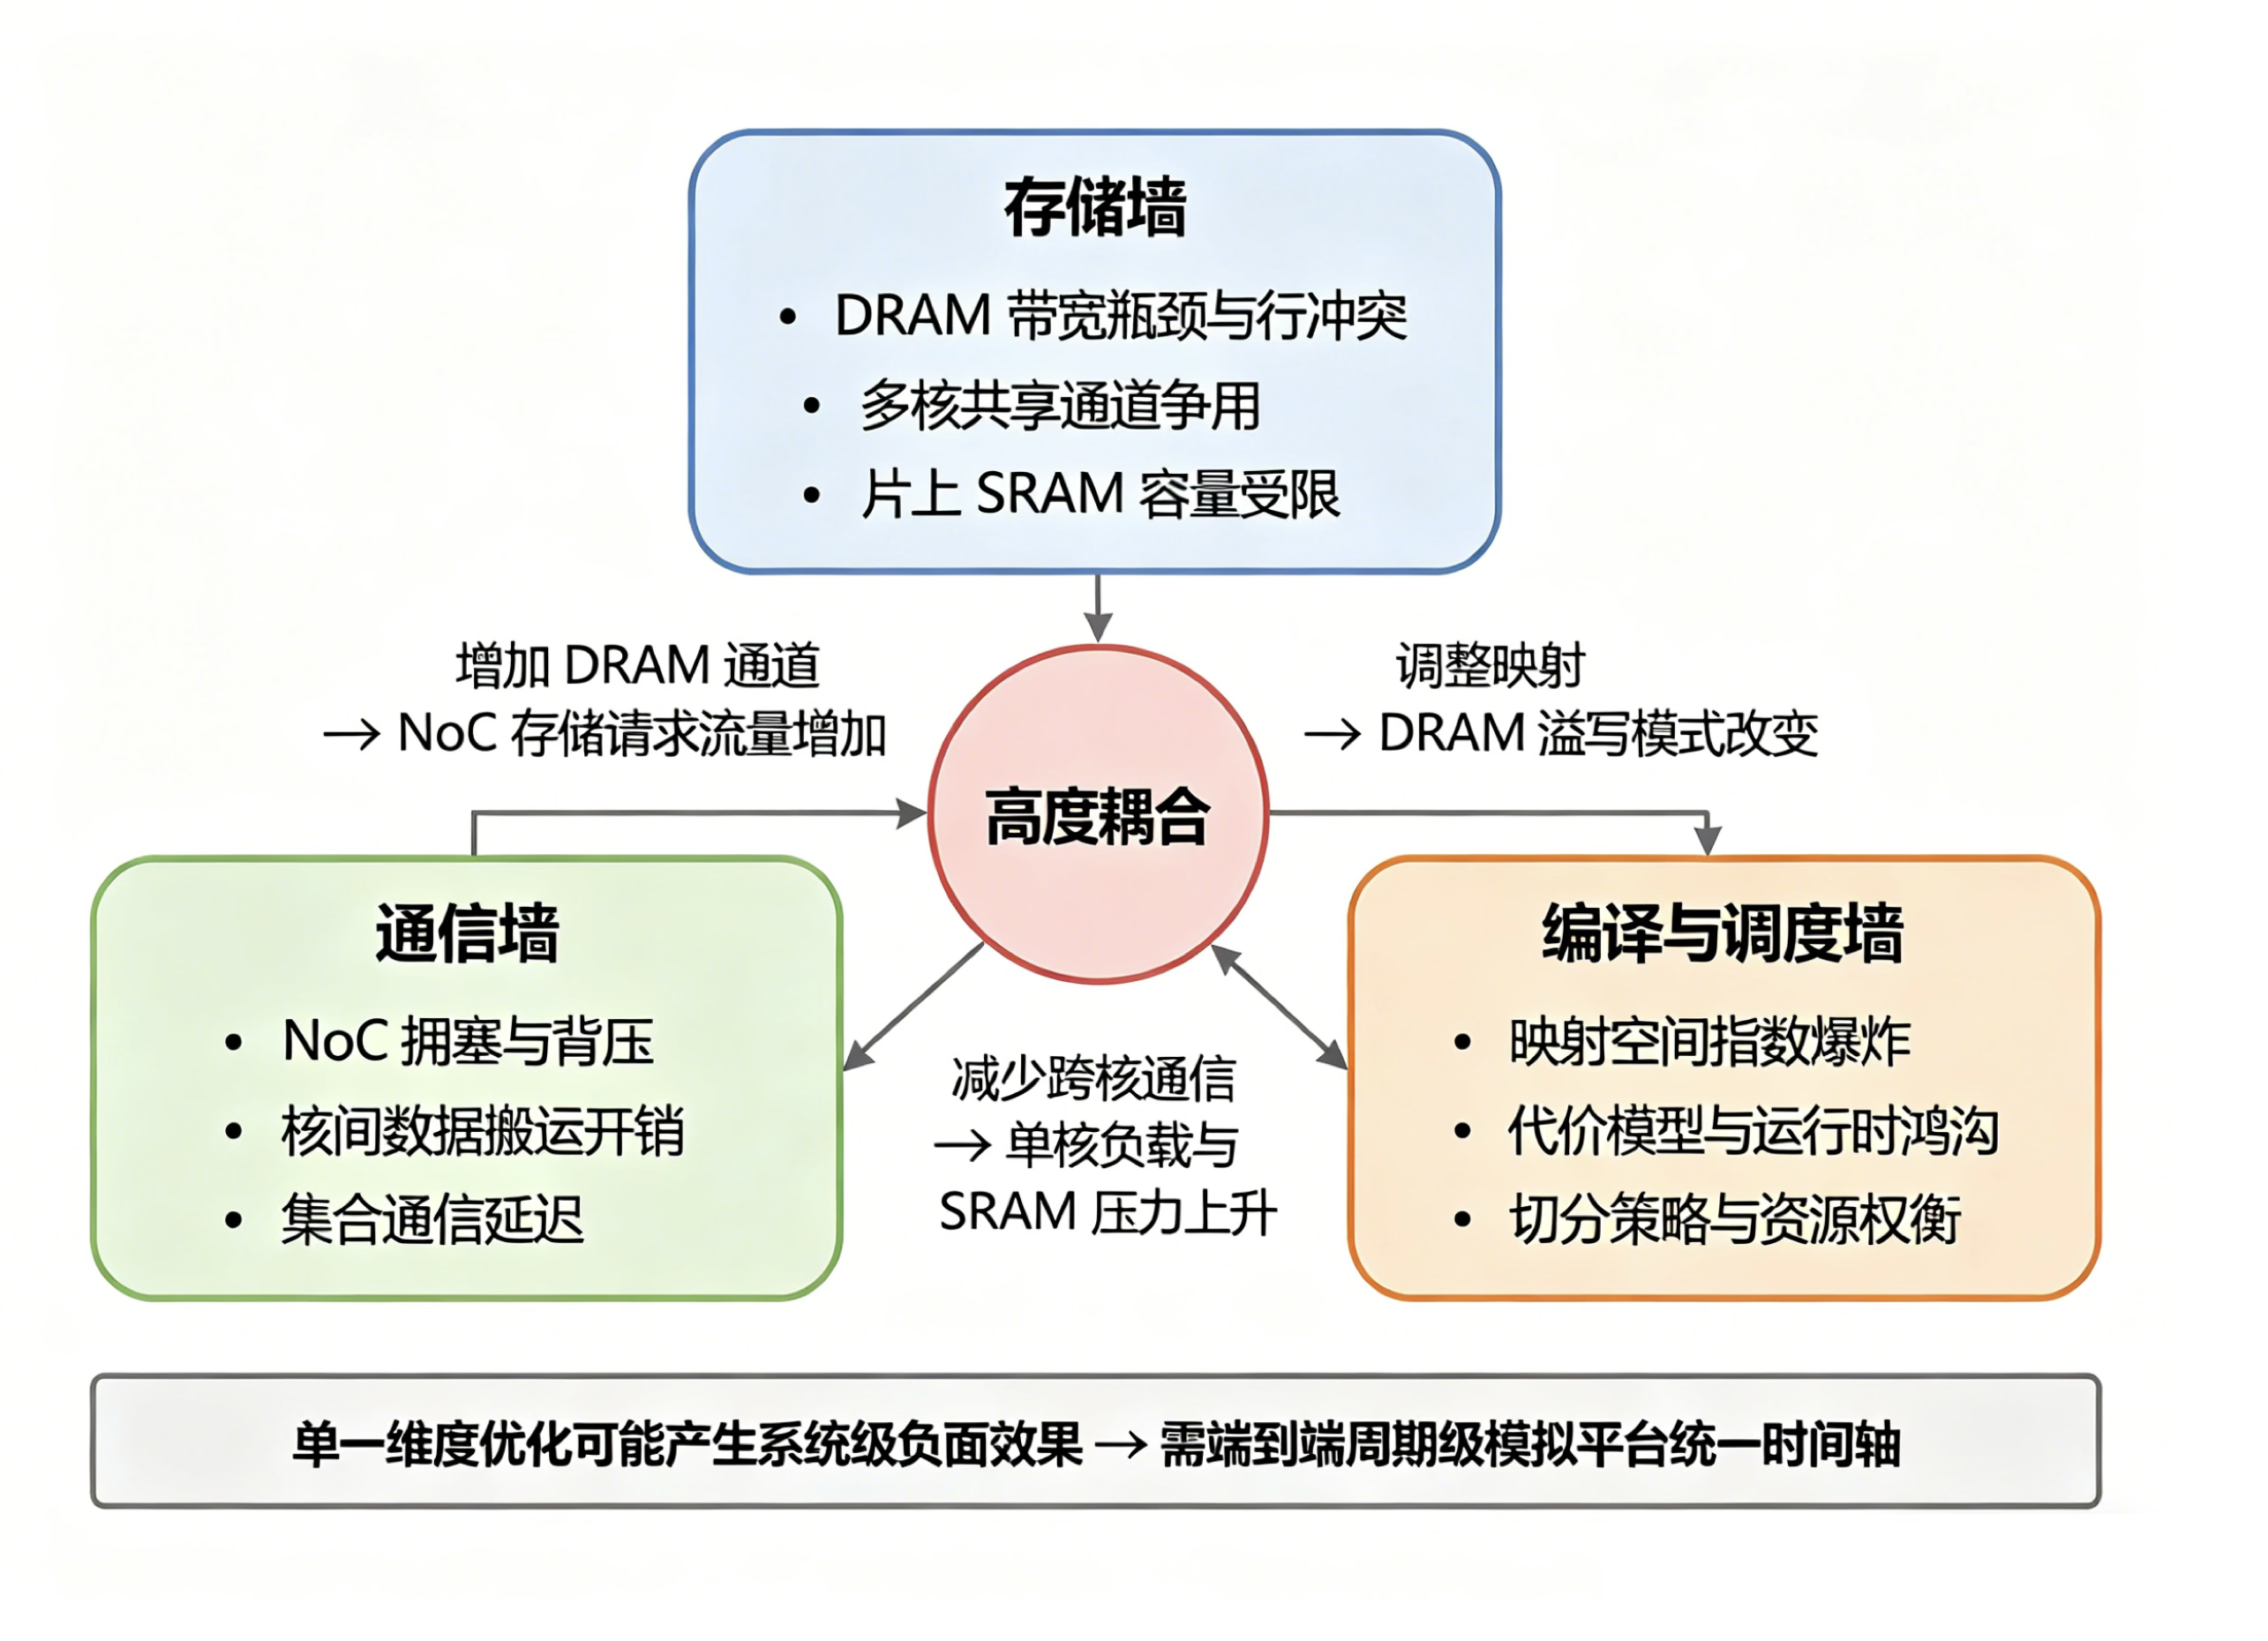
\includegraphics[width=\textwidth]{Figures/c1_three_walls.png}
  \caption{多核神经网络芯片面临的“三墙”及其耦合关系示意图}
  \label{fig:c1_three_walls}
\end{figure}
\vspace{-0.8em}

\xsection{国内外研究现状}{Related Work}

\xsubsection{神经网络芯片模拟器}{Neural Network Chip Simulators}

在多核架构下，模拟器不仅是验证正确性的工具，更是软硬件协同设计的核心引擎。图\ref{fig:c1_sim_role} 简要给出了多核神经网络芯片模拟器在架构探索中的作用示意，同时也是本篇工作提出的模拟器的工作流程图。模拟器接收上游编译/调度器生成的中间表示（Intermediate Representation, IR，包含工作负载与数据依赖）以及底层硬件架构参数（如计算单元数量、片上静态随机存取存储器容量、片上互连拓扑与主存带宽等）作为输入。在统一的时间轴下，模拟器驱动计算核心、片上网络（NoC）与片外存储（DRAM）协同推进，并输出端到端总周期、阶段分解统计（计算、通信、访存等待占比）以及资源利用率等定量指标。基于这些反馈，架构师与编译器开发者可以形成闭环优化：例如当发现访存等待占比过高时，可调整存算配比（增加 SRAM 或 DRAM 通道）。当发现网络背压严重时，可优化互连拓扑与路由。或者反馈给调度器以改进数据切分与映射策略。

\begin{figure}[htbp]
  \centering
  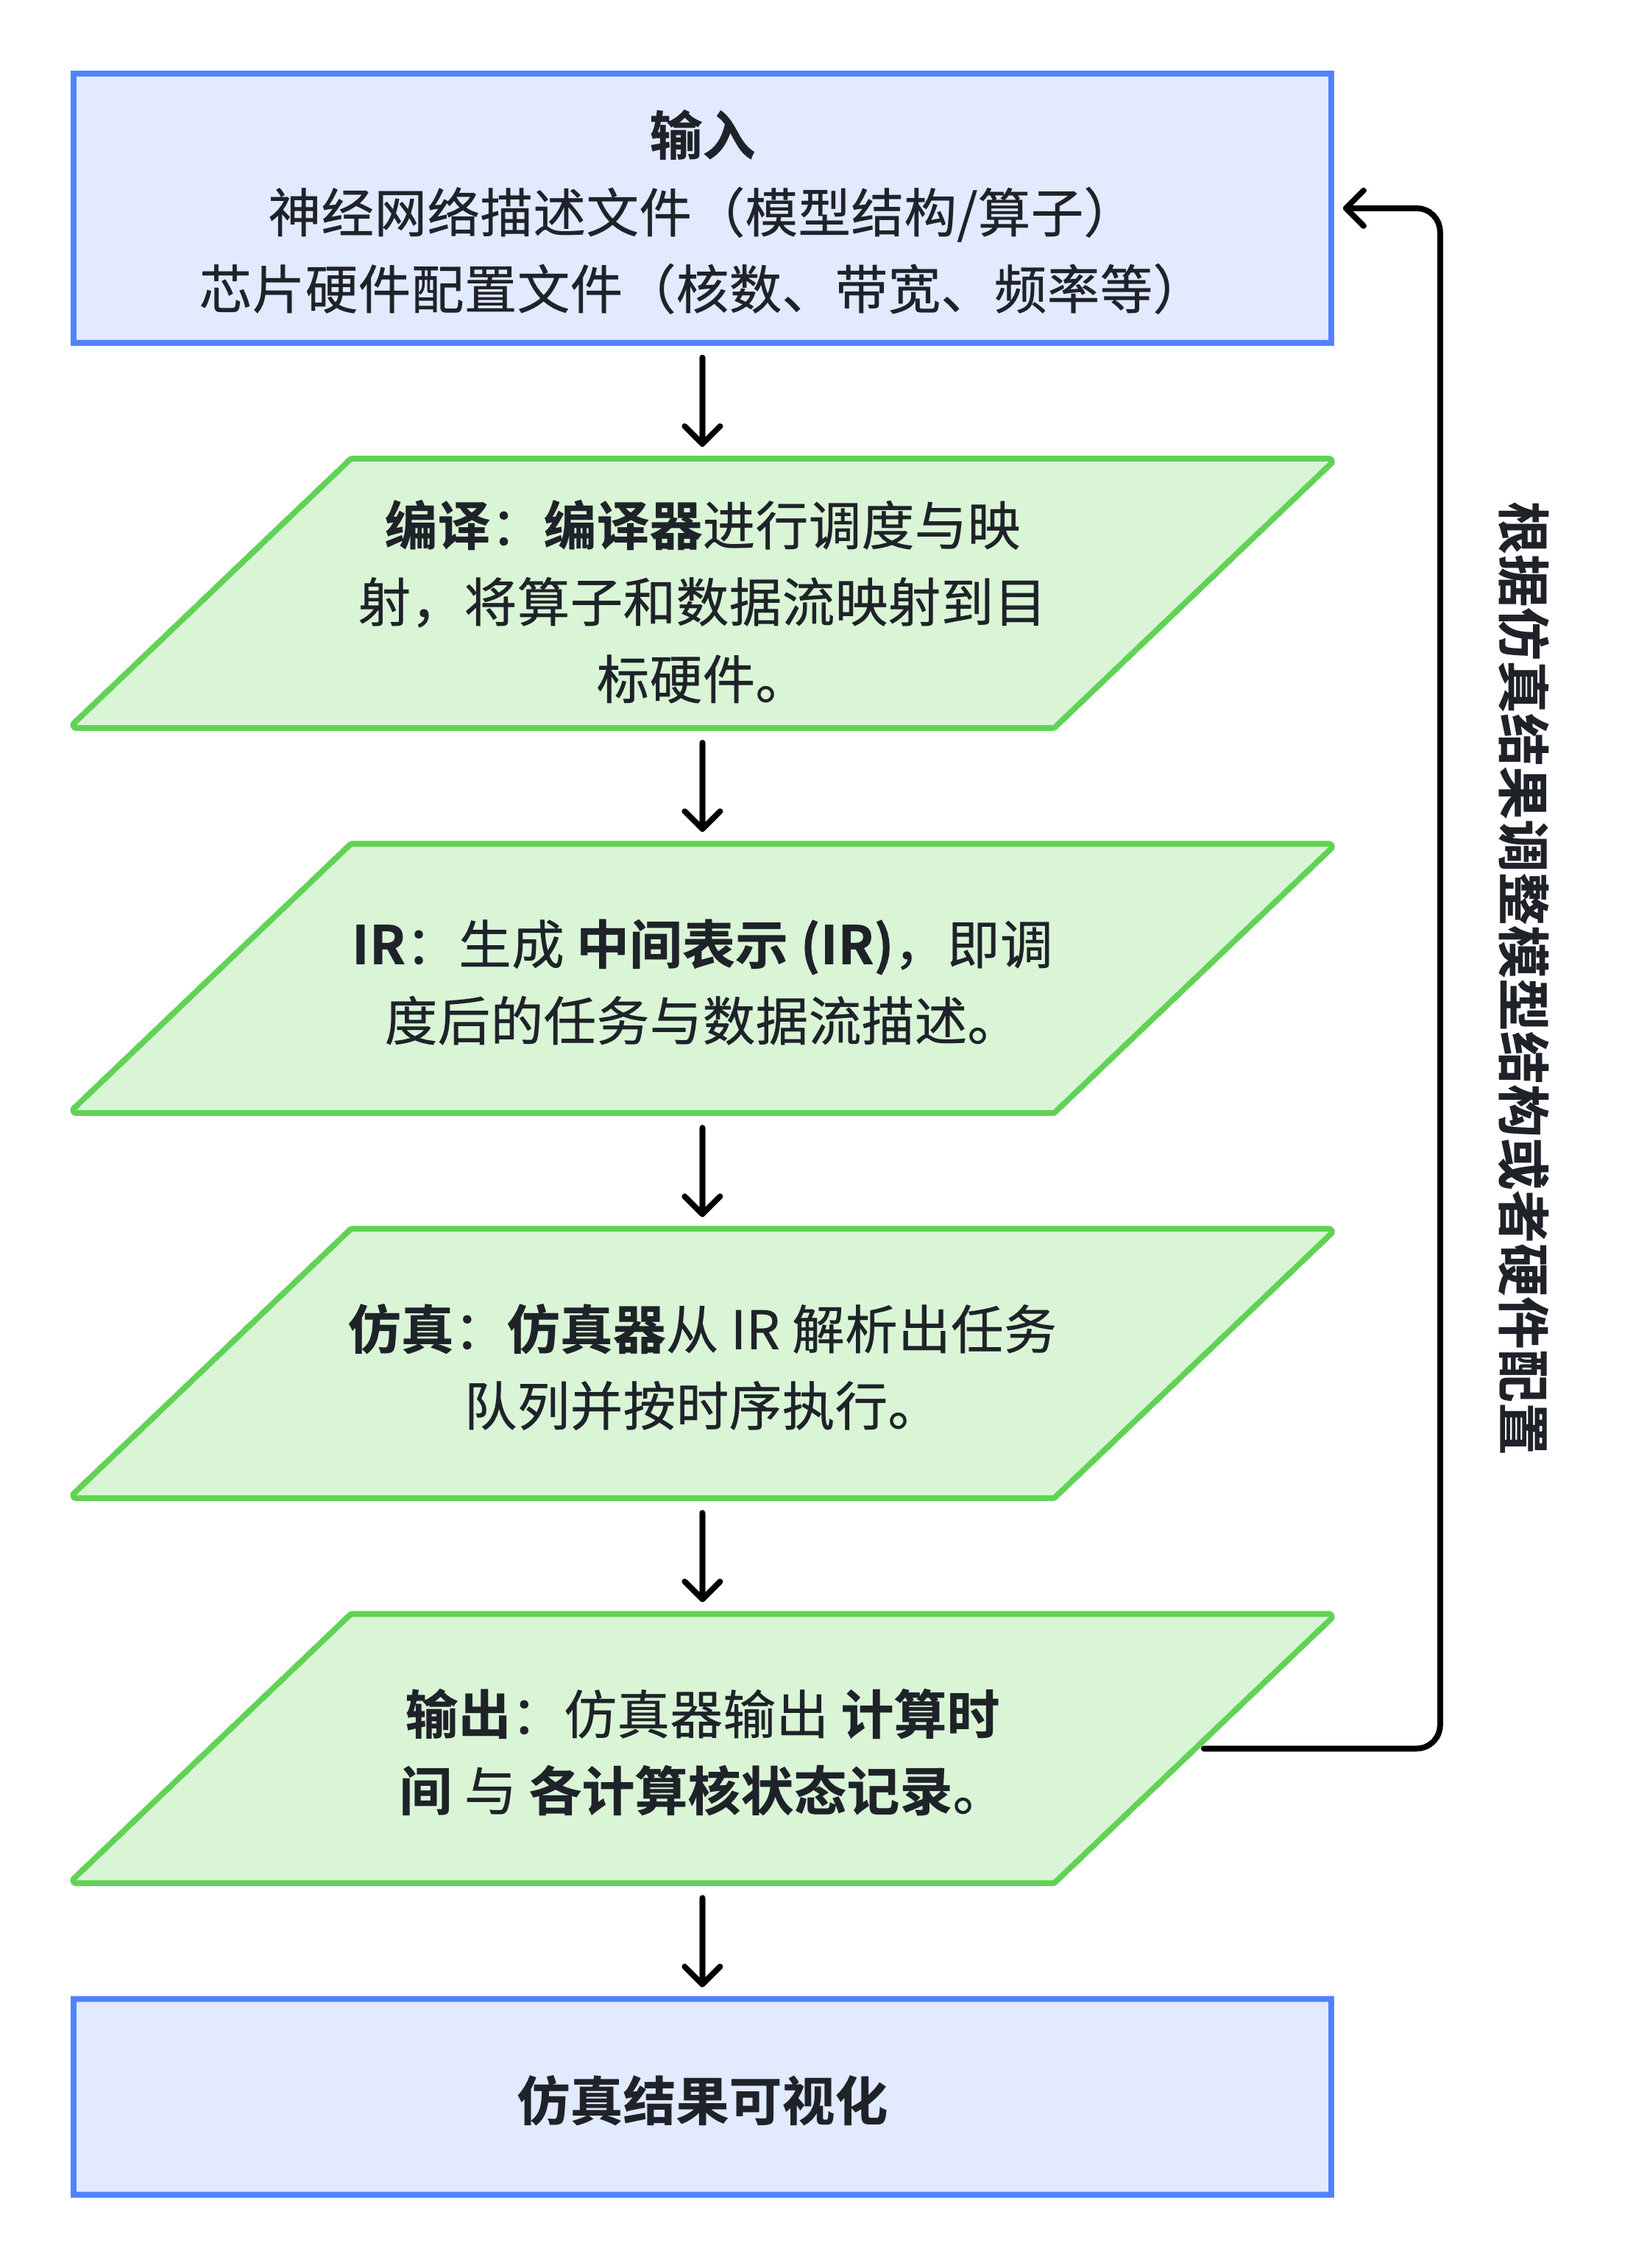
\includegraphics[width=0.55\textwidth]{Figures/workflow.png}
  \caption{多核神经网络芯片模拟器工作流程图}
  \label{fig:c1_sim_role}
\end{figure}

面向神经网络加速器的模拟与评估工具，按建模抽象层次与覆盖范围可大致分为三类：（1）以计算阵列数据流与复用分析为核心的解析模型，关注峰值吞吐、利用率与能耗等一阶指标。（2）兼顾片上存储层次、调度映射与互连行为的架构级周期模拟器，能够反映算子级到层级的运行时开销。（3）将编译栈、调度器输出与系统级时序打通的端到端模拟框架，支持在统一时间轴上观察多核、多时钟域与存储争用等耦合效应。不同层次的工具在建模精度、仿真速度与集成复杂度之间各有取舍，难以被单一工具同时满足。

在解析与数据流层面，早期研究多聚焦于单颗加速器或单一脉动阵列。文献\parencite{chen2016eyeriss}提出的 Eyeriss 加速器从片上数据复用与能效出发，系统研究了卷积数据流（如权重固定、输出固定、行固定）对能耗的影响，为后续数据流分类与评估奠定了基础。文献\parencite{jouppi2017tpu}介绍的 Google TPU 公开了首款大规模部署的云端推理脉动阵列设计与实测数据，确立了指令受限、计算受限与存储受限的系统级分析范式。文献\parencite{veronesi2021nvdla}介绍的 NVDLA 是开源的推理加速器知识产权核（Intellectual Property Core，IP Core），提供了从硬件寄存器传输级（Register Transfer Level，RTL）到编译栈的参考实现，为学术界研究软件栈与硬件行为链路提供了可复现的对象。在上述硬件参考平台之上，文献\parencite{samajdar2020scalesim}提出的 SCALE-Sim 工具针对脉动阵列数据流给出了轻量级周期级估算方法，可快速枚举不同数据流配置下的利用率与访存需求，广泛用于数据流与阵列规模的早期评估。文献\parencite{kwon2019maestro}提出的 MAESTRO 框架进一步以数据为中心描述深度神经网络（Deep Neural Network，DNN）在可配置加速器上的数据复用、延迟与能耗，为数据流驱动的解析评估提供了统一抽象。文献\parencite{gao2017tetris}提出的 TETRIS 则把 3D 存储与加速器数据流放在同一优化闭环中分析，揭示了带宽/容量层次对算子性能的关键影响。这一类工作普遍以解析模型或周期级乘法累加（Multiply-Accumulate，MAC）计数为主要手段，在算子级或网络层级提供性能上界分析。然而，其对多核 NoC 竞争、DRAM 排队与跨核同步等动态系统级行为的刻画能力有限。当多核规模扩展到十核乃至数十核时，其假设的近理想带宽利用与零争用条件与真实系统行为偏离较大\cite{ding2020survey}。

在架构级与系统级模拟层面，随着多核神经网络芯片与异构 SoC 逐渐成为主流，研究者开始把片上网络、片外存储与多核同步纳入统一的模拟闭环。文献\parencite{jin2024onnxim}提出的 ONNXim 模拟器针对多核神经网络芯片设计了周期级模拟流程，重点刻画多核与多租户场景下 NoC 与 DRAM 的竞争行为，能够对端到端延迟与吞吐进行定量评估，为多核神经网络芯片的系统级瓶颈分析提供了可用的工具基础。在更广泛的系统级模拟领域，文献\parencite{zhang2023gem5nvdla}介绍的将通用处理器模拟框架 gem5 与 NVDLA 加速器模型相结合的工作，实现了从编译、调度到系统执行的端到端链路，为软件栈与硬件行为的一体化评估提供了参考架构。此外，近年来针对稀疏化、流式张量与新型数据流的模拟工作（如文献\parencite{set2023isca}提出的基于张量抽象的事件驱动模拟器），也拓展了模拟器在新兴算子形态与编译策略下的适用范围。这类工作相对解析模型提供了更贴近真实行为的系统级指标。然而，它们在编译/调度器的输入接口、子模块可插拔性以及可解释统计输出等工程能力上仍存在欠缺，较难直接服务于一次改映射、一次改硬件配置的高频迭代场景。

综合国内外现状，面向多核神经网络芯片架构探索与编译协同的周期级模拟工具仍存在三方面典型不足。第一，上游编译/调度器输出的 IR 与模拟器输入格式往往脱节。模拟器多依赖自定义的踪迹或简化的工作负载描述，无法直接消费调度器生成的、带有显式依赖与数据流向的 IR。这一脱节导致每次更新映射都需重新构造模拟输入，迭代成本高且难以保证语义一致。第二，NoC 与 DRAM 子系统的建模多为内置固定实现，缺少统一的抽象接口与可插拔后端设计。研究者难以在不改动核心执行逻辑的前提下替换不同精度的后端（如简单延迟模型与周期级 NoC/DRAM 模拟器）或更换不同配置进行对照实验，设计空间探索的变量隔离性不足。同时，子模块的版本升级与替换往往牵连大量执行层代码改动，制约了工具链的可演化性。第三，模拟输出多为端到端总周期或简单分类统计，缺乏与计算、通信与存储阶段一一对应的可解释指标（如每核不同状态时间占比、显式 NoC 背压周期、DRAM 请求排队周期等）。这种粗粒度输出既不利于瓶颈归因与架构参数敏感性分析，也不利于把模拟结果直接反馈给调度器以驱动映射改进。本文针对上述三方面不足，设计以调度器 IR 为输入的端到端模拟流程。在执行层之外，面向异构子模块模拟器构建松耦合 NoC/DRAM 接口，并建立可复现的阶段分解与热点统计体系。这一组件构成涵盖 IR 输入、周期级执行与可解释输出的模拟基础设施，为多核神经网络芯片的系统级研究提供了支撑。

\xsubsection{任务调度与编译优化}{Task Scheduling and Compilation Optimization}

神经网络在神经网络芯片上的高效执行依赖编译与调度两端的协同：编译器负责算子融合、数据布局与循环变换，调度与映射则决定计算与数据在空间（多核）与时间（流水、批处理）上的分配。这两端的决策相互耦合——循环变换的可行性受限于硬件数据流与片上存储容量，而映射的优劣又取决于编译器所暴露出的并行度与复用机会——因而现代神经网络芯片编译栈往往需要在图级、算子级与映射级之间建立端到端的可评估闭环。

在编译基础设施方面，文献\parencite{lattner2021mlir}提出的多层中间表示框架（Multi-Level Intermediate Representation，MLIR）为领域专用后端提供了可扩展的方言（Dialect）与变换管道。这种设计使得从高层图表示到硬件相关指令的逐层下译（Lowering）过程更加模块化与可复用。面向具体神经网络芯片的编译栈在此基础上不断丰富，例如文献\parencite{qualcomm2026hexagonmlir}介绍的面向高通 Hexagon NPU 的 MLIR 编译栈，展示了从模型到神经网络芯片指令的完整链路及在真实硬件上的优化实践。在更通用的编译框架层面，文献\parencite{chen2018tvm}提出的 TVM 框架以张量表达式与学习式代价模型为核心，并结合 AutoTVM/Ansor 等自动调度机制。该框架在多种加速器与 GPU 上实现了算子级的跨平台优化，为自定义神经网络芯片后端提供了可借鉴的调度语言与搜索算法。上述工作主要侧重单核或单芯片内的算子优化与指令生成，对多核映射与跨核数据流的形式化描述相对较少。同时，其代价模型多以峰值算力与理想带宽为基础，难以刻画多核 NoC 与 DRAM 的动态行为。

在映射与调度层面，多核场景下的空间划分与流水编排是一个组合优化问题，搜索空间随核心数与网络深度快速增长。文献\parencite{parashar2019timeloop,wu2019accelergy}提出的 Timeloop 与 Accelergy 为加速器映射与能耗建模提供了一套以循环嵌套变换为核心的分析方法，被广泛用于单核与多级存储层次上的映射枚举。文献\parencite{huang2021cosa}提出的 CoSA 将映射问题形式化为约束优化并用求解器在合法映射空间中搜索近优解。文献\parencite{yang2020interstellar}提出的 Interstellar 借用 Halide 的调度语言描述 DNN 到加速器的映射，通过系统化枚举数据复用与并行策略分析设计空间。面向更大规模的多核/多芯片系统，文献\parencite{cai2024gemini}提出的 Gemini 调度器将层流水与空间映射编码为统一的表示（Layer-Pipeline Spatial Mapping），并采用动态规划算法与模拟退火算法在映射空间中搜索，从而实现了在多核架构上对映射与架构参数的联合探索。该调度器的输出以结构化 IR 描述各核工作负载及其依赖关系。近年来，面向缓存与片上存储的分配策略也出现了专门化的优化工作。文献\parencite{set2023isca}提出的 SET 通过系统化的张量切分与存储规划提升利用率，文献\parencite{bufferprospector2024}提出的 BufferProspector 从缓冲分配角度系统分析并搜索片上存储的最优方案。这一系列工作显示出调度、映射与存储分配的联合优化正在成为新的研究重点。

然而，上述映射与调度方法普遍依赖对执行代价的估计以驱动搜索。其代价模型通常基于峰值算力、理想带宽与固定延迟等简化假设，难以反映实际运行时的 NoC 拥塞、DRAM 排队与行冲突等多核系统级效应。因此，映射与调度算法的有效性往往需要在更贴近真实系统行为的模拟环境中二次验证。若模拟器无法直接消费调度器 IR 并反馈周期级指标，则只能通过事后踪迹注入或手工改写输入进行间接评估，迭代效率与结论可信度均受限，难以形成调度搜索、模拟评估与反馈改进的短周期闭环。本文通过 IR 驱动、闭环执行的设计，使调度器输出可直接驱动模拟并得到阶段级统计与可解释的瓶颈归因，为编译、调度与架构的协同优化提供可复用的评估闭环。

\xsubsection{互连与存储优化}{Interconnect and Memory Optimization}

多核神经网络芯片的端到端性能受片上网络与片外存储的时序与竞争行为影响显著，相关研究依赖高保真的 NoC 与 DRAM 建模工具，并需要把二者与计算核心的执行时序在同一时间轴下对齐，才能反映真实系统中的争用、排队与背压传播等动态效应。

在片上网络方面，文献\parencite{jiang2013booksim}提出的 BookSim 模拟器及其后续版本 BookSim2 被广泛用作周期级 NoC 模拟器。该模拟器支持二维网格 Mesh、环面 Torus、胖树 Fat-Tree 等多种拓扑，支持 XY 维序路由与自适应路由等多种路由算法，并提供虚拟通道数、缓冲深度以及分片与数据包划分等可配置维度。其能够刻画链路仲裁、排队与尾延迟等拥塞效应，是 NoC 研究中事实上的参考工具。近年来，面向高带宽与多流并行的开源 NoC 设计（如文献\parencite{flooonoc2024}提出的 FlooNoC）在物理层与协议层提供了可配置的互连模型，为集成到全系统模拟中提供了可选组件。这类工具在单独使用时，通常接受合成流量（如均匀随机、热点、置换流量）或由其他工具生成的数据包级踪迹（Packet-Level Trace）作为输入。它无法根据神经网络芯片核心的实时执行状态动态产生请求，因而难以体现计算完成、发起传输与对端消费之间的依赖链与背压传播。在多核神经网络芯片场景下，NoC 与计算和存储的耦合评估仍依赖上层模拟框架把核心状态、读写事务与 NoC 推进过程统一组织起来，这对模拟器的集成能力与接口抽象提出了较高要求。

在片外存储方面，DRAM 的时序约束、存储体（Bank）并行度与调度策略对有效带宽影响巨大。文献\parencite{luo2023ramulator2}提出的 Ramulator2 模拟器以模块化与可扩展的方式实现了多种 DRAM 标准的时序与调度建模，所支持的标准包括 DDR3、DDR4、LPDDR 与 HBM 等。该模拟器支持行缓冲、刷新策略以及先就绪先到先服务（First-Ready First-Come-First-Served，FR-FCFS）等多种调度算法，使排队延迟、行命中率与冲突行为可在模拟中复现。在多核神经网络芯片中，多个核心并发访问 DRAM 时共享通道与 Bank，请求交织与行冲突会使实际带宽远低于标称峰值。这种带宽损失对通道数、Bank 数、地址映射策略等参数高度敏感。若叠加以大模型推理所特有的权重/KV Cache 密集访存特征，这一矛盾在吞吐与延迟两端都会被进一步放大\cite{gholami2024aimemorywall}。只有将 DRAM 模型与多核执行时间轴对齐的周期级模拟，才能系统性地评估这类动态效应在不同架构配置下的表现。

此外，面向多核神经网络芯片的互连与存储研究还表现出若干值得关注的新趋势：（1）存储墙问题推动了片上存储层次的精细化建模与搜索，如缓冲分配与张量切分的联合优化\cite{bufferprospector2024,set2023isca}。（2）高带宽片外存储（如 HBM）在云端与高端推理平台上的普及，使得研究者需要在模拟中区分 DDR、LPDDR 与 HBM 等不同标准在带宽、延迟与并行度上的差异。（3）计算与通信的耦合评估越来越强调事件驱动的逻辑：即请求的发起时刻不再独立于核心执行，而必须由核心状态机在运行时动态触发，以真实反映依赖闭环。

综合来看，NoC 与 DRAM 的优化若脱离具体映射与负载特征进行孤立分析，难以反映端到端效果。若要与映射和调度联动评估，又需要统一的模拟平台在相同时间基准下驱动 NoC 与 DRAM 请求、并汇总可解释的阶段级统计。然而，现有模拟框架大多将 NoC/DRAM 后端以硬编码方式嵌入执行层，难以在不改动核心代码的前提下切换不同后端或不同精度模型。这一限制阻碍了先用简单模型快速迭代、再用高保真模型精细评估的分层研究路径。本文针对这一痛点，定义 NoC 子系统与 DRAM 内存子系统的松耦合接口，并将 BookSim2 与 Ramulator2 封装为可插拔后端。该设计在保持执行层逻辑不变的前提下，支持简化后端与高保真后端的对照实验与设计空间探索，弥补了互连与存储优化研究与多核神经网络芯片端到端评估之间的衔接不足。

\xsubsection{软硬件协同设计与评估}{Hardware-Software Co-design and Evaluation}

随着神经网络芯片在架构参数空间（如处理单元数量、片上缓存容量、互连带宽等）与软件映射空间（如数据流策略、层间调度、算子融合等）上的设计选择日益增多，软硬件协同设计（Hardware-Software Co-design）成为兼顾性能与效率的关键方法论。其核心思想在于，将算法、编译映射与硬件架构作为统一的优化空间进行联合探索，而非在固定硬件上优化软件或在固定映射下搜索硬件参数。

在预 RTL 阶段的快速架构评估方面，文献\parencite{shao2014aladdin}提出的 Aladdin 工具基于动态数据依赖图实现了预 RTL 加速器性能与功耗模拟方法，能够在不编写 RTL 的前提下对定制加速器进行大规模设计空间探索。文献\parencite{samajdar2020scalesim}提出的 SCALE-Sim 工具对脉动阵列的不同数据流配置进行快速周期估算，为硬件参数与映射的联合评估提供了轻量级工具。这类工作通过降低评估成本来扩大可搜索的设计空间，但多聚焦于单核或单个计算阵列，对多核 NoC 争用与共享存储竞争的建模有限。

在映射与架构的联合搜索方面，前述 Gemini、Timeloop/Accelergy、CoSA 与 Interstellar 等工作在编译映射与硬件参数之间建立了定量关联。然而，其评估所依赖的代价模型多为解析模型或简化的周期估计，难以体现 NoC 拥塞、DRAM 行冲突等多核系统级效应。

在算法与硬件的端到端联合优化方面，文献\parencite{wu2019fbnet}提出的硬件感知神经网络架构搜索（Hardware-aware Neural Architecture Search，NAS）方法在搜索网络结构时将目标硬件的延迟或能耗纳入评估函数，使搜索结果能同时满足精度与部署约束。与之类似的能效评估工作也在神经网络芯片的高能效单元设计层面不断深入，例如文献\parencite{soma2024}对低功耗计算单元与神经网络芯片结合的架构探索。但这类方法通常以固定硬件平台或预设代价模型为前提，对硬件侧的参数可调性与系统级动态行为考虑不足。当硬件架构本身也处于探索阶段时，仍需模拟器提供对不同架构配置下的执行代价估计与瓶颈归因。

另一个影响协同设计评估质量的关键因素，是评估对象粒度与优化对象粒度的匹配程度。若评估工具仅能给出端到端总周期或简单的计算/通信/存储三分类，则在多核神经网络芯片这类多维耦合系统中，研究者难以判断某次改动究竟改善了哪一环节、又是否引入了新的瓶颈。近年来 Sze 等人在综述中指出\cite{sze2017efficient}，高效神经网络硬件的设计与评估必须覆盖算子、数据流、存储层次与互连等多个抽象层次，并要求评估工具能够对其中每一层提供可解释的量化指标。这对模拟器在统计输出上的工程设计提出了超出总周期正确性的更高要求。

综上，软硬件协同设计的有效性高度依赖评估工具在精度、效率与可解释性三者之间的平衡。解析模型速度快但精度受限于静态假设。RTL 仿真精度高但迭代成本过大。周期级模拟器——特别是能够直接消费编译/调度输出并在统一时间轴下反映多核系统行为的端到端模拟平台——填补了二者之间的精度与效率空白，为改映射或改架构后快速得到可信反馈的协同优化循环提供了必要的基础设施。本文所设计的模拟器正是面向这一需求，以 IR 为输入统一编译与模拟的接口、以松耦合抽象支持子系统后端可插拔、以阶段级统计与热点可视化提升结果可解释性，使软硬件协同探索具备低迭代成本与可信的定量依据。与解析类工具相比，本文模拟器在牺牲一定速度的前提下补全了 NoC 背压与 DRAM 争用等系统级行为的刻画。与完整 RTL 或硬件模拟平台相比，本文模拟器在牺牲一定精度的前提下换取了远低于硬件流程的迭代成本与更丰富的可观测性，从而在多核神经网络芯片架构探索与编译协同场景下占据一个独特的定位。

\xsubsection{当前研究存在的问题}{Open Problems}

综合 1.2 节对国内外研究现状的综述，可以看到神经网络芯片模拟器、编译调度、互连存储与软硬件协同等方向均已积累了较为丰富的研究成果。然而，面向多核神经网络芯片端到端周期级评估的研究链条，在以下三方面仍存在共性不足，构成本文的研究问题。

问题一：上游编译/调度器输出的 IR 与模拟器输入接口脱节。已有多核模拟器多依赖自定义踪迹或简化的工作负载描述，无法直接消费调度器生成的、带有显式依赖与数据流向的结构化 IR。每次更新映射策略都需要重新构造模拟输入，迭代成本高且难以保证语义一致。这使调度搜索、周期级评估与反馈改进的闭环难以在低成本下闭合。

问题二：NoC 与 DRAM 子系统接口硬编码、可插拔性差。多数模拟器将 NoC 与 DRAM 模型嵌入执行核心，研究者难以在不改动核心执行逻辑的前提下替换为不同精度或不同配置的后端。设计空间探索的变量隔离性因此不足，且子模块的版本升级与替换牵连大量执行层代码改动，制约了工具链的可演化性。

问题三：模拟输出粒度粗、瓶颈归因能力弱。已有工具多输出端到端总周期或简单的计算/通信/存储三分类，缺少与计算、NoC 背压与存储等待阶段一一对应的可解释指标（如每核状态时间占比、显式 NoC 背压周期、DRAM 请求排队周期等）。这种粗粒度输出既不利于瓶颈归因与架构参数敏感性分析，也不利于把模拟结果直接反馈给调度器以驱动映射改进。

针对上述三方面问题，本文设计并实现了一个 IR 驱动、松耦合、可解释的端到端多核神经网络芯片周期级模拟平台，具体研究内容与创新点见下文。

\xsection{研究内容与创新点}{Research Content and Innovations}

\xsubsection{本文主要工作}{Main Work}

本文围绕面向芯片早期设计阶段的端到端周期级多核神经网络芯片模拟平台的构建与利用展开。该平台以工作负载为最小执行单元，在统一时间轴上刻画计算、通信与存储三者的系统级争用，以支持流片前的架构参数与映射策略快速扫描，而不追求指令级或寄存器传输级的核内精度。围绕该定位，本文在平台设计、系统集成与实验验证三方面开展研究，具体研究内容与所做工作如下。

（1）端到端模拟框架的设计与实现。 以文献\parencite{cai2024gemini}提出的 Gemini 调度器生成的结构化 IR（JSON 格式）为芯片工作负载输入，以芯片描述文件为可配置参数，设计并实现从IR解析到周期级执行、再到统计与踪迹输出的完整模拟流程。模拟引擎在统一全局周期下推进多颗计算核心。每核按依赖到齐、计算与写回的语义执行工作负载，并通过拉取式数据流与片上网络、片外存储交互。其中，核间数据依赖经由 NoC 请求/响应完成，与 DRAM 的读写经由存储接口完成。计算、通信与存储三者共享同一时间轴，从而能够刻画排队、背压与资源争用对端到端周期的影响。为支持不同精度的评估需求，NoC 与 DRAM 均抽象为统一接口，并提供简化后端与基于 BookSim2、Ramulator2 的高保真后端两种实现。该设计支持在不修改执行层逻辑的前提下切换或对照，便于设计空间探索时的变量隔离与可复现对比。

（2）统一任务抽象与可配置核心建模。 将上游 IR 中的核心网格、每核工作负载序列及数据依赖解析为与格式无关的统一任务表示，执行层仅依赖该抽象，从而实现内容与形式分离，在 IR 格式演进时仅需扩展解析器。单核执行采用依赖驱动的五态状态机建模，核心计算能力与本地 SRAM 容量均参数化配置（如乘加器数量、向量处理器单元数量、SRAM 容量），以支持后续对计算资源与存储配置的扫描实验。在多时钟域场景下，通过全局周期与可配置的 DRAM 时钟频率实现多速率推进，在保证因果一致的前提下刻画计算核心/片上网络与 DRAM 频率差异对端到端性能的影响。

（3）基于模拟器的实验验证与分析。 为体现模拟器的实用价值，本文在模拟平台上开展从精度验证、多核瓶颈分析到设计空间探索的系统性实验。微基准与 ZeBu 对照：通过片上网络同步实验（双核点对点依赖）与内存同步实验（仅 DRAM 依赖）验证依赖因果、核间通信与 DRAM 闭环及子模块使用不同后端差异。与 Synopsys ZeBu 硬件模拟平台对比单核模拟结果，将相对误差控制在 $\pm$5.2\% 以内。真实 AI 负载瓶颈与热点分析：以调度器生成的残差网络（Residual Network，ResNet）系列模型 ResNet34、ResNet50 的 IR 驱动模拟，对端到端周期进行阶段分解（计算、NoC 背压、存储等待），并辅以各核阶段占比热力图等可视化，实现可解释归因。多核瓶颈分析与递进式优化：在四核配置下，以 ResNet50 为负载，构造存储受限基线（DDR4 单通道）。通过两步递进式优化逐级缓解瓶颈，先将 DRAM 由 DDR4 升级到 HBM 四通道，使峰值带宽提升约 6.7 倍，再将 SRAM 端口由 256 加宽至 \SI{1024}{B/cycle}。优化后总周期由 238,803 降至 62,818，加速比达到 3.80 倍，瓶颈也由 DRAM 带宽逐级迁移到 SRAM 端口带宽。多核吞吐量设计空间探索：沿单核算力、核数扩展与批量三个维度展开 12 组配置仿真，其中单核算力按乘法累加单元（Multiply-Accumulate，MAC）数量取 256、512、1024 三档，核数取 4、16、64，批量（Batch Size）取 1、4。实验给出若干定量结论：存储受限状态下提升 MAC 算力无效，核数超过负载并行度上限后性能反而退化（64 核出现死锁），批量扩展效率仅约 24\%。这些结论为芯片设计前期的参数定界提供了快速反馈依据。

综上，本文一方面完成了模拟平台从 IR 输入到周期级输出到多时钟同步的完整设计与实现。另一方面基于该平台开展了从精度验证、瓶颈归因到多维设计空间探索的系统性实验。两者结合使模拟器不仅作为多核神经网络芯片研究的评估工具，也通过具体实验体现其在正确性校验、瓶颈定位与架构参数优化中的实际价值。

\xsubsection{本文创新点总结}{Innovations Summary}

本文的创新点主要体现在以下三方面。

第一，设计并实现了一套面向多核神经网络芯片的端到端周期级模拟器，并通过对照实验验证了精度。模拟器填补了硬件模拟器和分析性软件模拟器之间的空白。

第二，模拟器采用可扩展的接口化结构，具有高通用性和高可扩展能力，可在不修改主体代码的前提下接入不同的模拟后端。

第三，提出了利用周期级模拟器分析芯片动态行为的瓶颈分析方法，提升了芯片早期参数定界和软硬件协同优化的效率。

\xsection{论文组织结构}{Thesis Organization}

本文共五章，按问题与现状、基础与工具、两项研究工作以及总结与展望的逻辑展开。

第一章为绪论。该章在研究背景与意义中阐述算力需求与神经网络芯片的发展脉络，并分析多核神经网络芯片的三墙挑战及其耦合关系。在国内外研究现状中，分别从神经网络芯片模拟器、任务调度与编译优化、互连与存储优化以及软硬件协同设计与评估四个方向综述代表性研究，并归纳当前研究存在的问题。随后阐述本文的主要工作与创新点，最后给出全文的组织结构。

第二章为软硬件基础与前置技术。该章介绍多核神经网络芯片体系结构、工作负载特征以及周期级模拟方法，并阐明 ZeBu、BookSim2、Ramulator2 的角色与集成方式。在此基础上说明编译与调度挑战，阐述调度器 IR 与模拟器的衔接，为后续两章研究工作做铺垫。

第三章为模拟器的设计与实现。该章围绕模拟平台本体展开。首先给出问题定义与设计目标，继而依次叙述模拟器整体架构、NoC/DRAM 松耦合接口、可配置计算核心建模与全系统同步机制的完整设计与实现。最后通过片上网络同步、内存同步与 ZeBu 对照三组实验，验证模拟器的因果一致性、DRAM 闭环正确性，以及与硬件模拟在真实负载上的总周期精度。

第四章为基于模拟器的瓶颈分析和设计空间探索。该章在第三章模拟平台的基础上展开两项实证研究。其一，建立基于阶段占比分解与按核可视化的归因方法，定位单核与多核场景下的端到端瓶颈。其二，沿单核算力、核数扩展与批量三个维度开展 12 组配置的设计空间探索。

第五章为结论与展望。该章对全文主要工作与所得结论做简要总结，并对未来研究方向进行展望。
